%%%%%%%%%%%%%%%%%%%%%%%%%%%%%%%%%%%%%%%%%%%%%%%%%%%%%%%%%%%%%%%%%%%%%%%%%%%%%%%%
\section{The Tutorial Scenario}

%%%%%%%%%%%%%%%%%%%%%%%%%%%%%%%%%%%%%%%%%%%%%%%%%%%%%%%%%%%%%%%%%%%%%%%%%%%%%%%%
\begin{frame}
    \frametitle{Outline}
    \begin{columns}[t]
        \begin{column}{.5\textwidth}
            \tableofcontents[sections={1-7},currentsection]
        \end{column}
        \begin{column}{.5\textwidth}
            \tableofcontents[sections={8-15},currentsection]
        \end{column}
    \end{columns}
\end{frame}

%%%%%%%%%%%%%%%%%%%%%%%%%%%%%%%%%%%%%%%%%%%%%%%%%%%%%%%%%%%%%%%%%%%%%%%%%%%%%%%%
\begin{frame}
	\frametitle{What is this about?}
	\begin{docs}[Objective]
		\begin{enumerate}
			\item Introduce to the Tutorial Scenario 
		\end{enumerate}
	\end{docs}
\end{frame}

\subsection{Tasksetting}

%%%%%%%%%%%%%%%%%%%%%%%%%%%%%%%%%%%%%%%%%%%%%%%%%%%%%%%%%%%%%%%%%%%%%%%%%%%%%%%%
\begin{frame}
  \begin{figure}
    \centering
    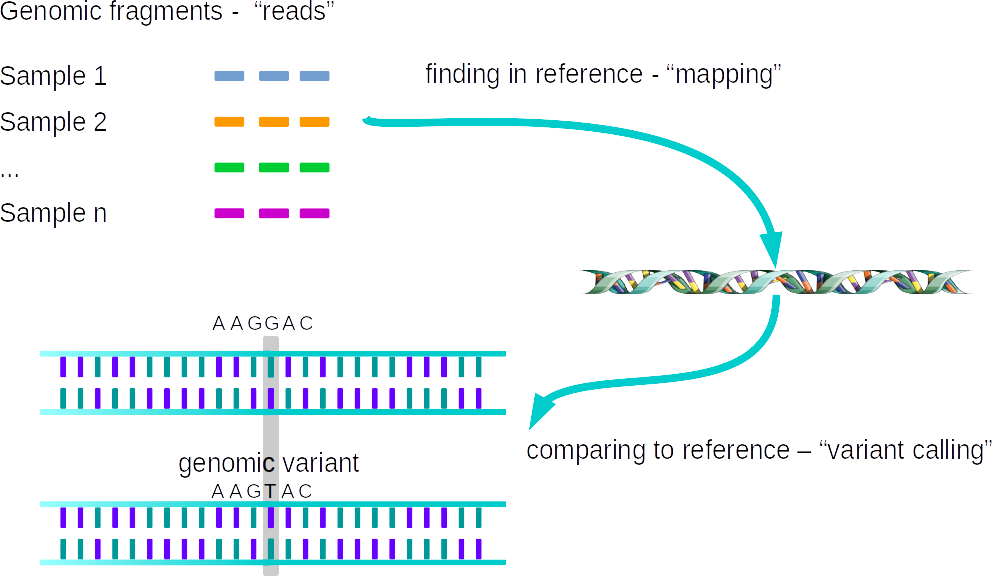
\includegraphics[width=0.95\textwidth]{biology/variant_calling_workflow.png}

    \smallskip

    \caption{\href{https://www.intechopen.com/chapters/53334}{Zhao, Watrous, Zhang \& Zhang (2016)}}
  \end{figure}
\end{frame}


%%%%%%%%%%%%%%%%%%%%%%%%%%%%%%%%%%%%%%%%%%%%%%%%%%%%%%%%%%%%%%%%%%%%%%%%%%%%%%%% 
\begin{frame}[fragile]
	\frametitle{\HandsOn{Obtaining Your Tutorial Sample Data}}
	Please run the \altverb{get_tutorial.sh} script you just copied:
	\begin{lstlisting}[language=Bash, style=Shell,basicstyle=\footnotesize]
$ bash get_tutorial.sh
	\end{lstlisting}
	\begin{task}
		This script will download and unpack the sample data for this course. Please take a look in this script to understand it. Where are your sample data after running this script?
	\end{task}
\end{frame}


